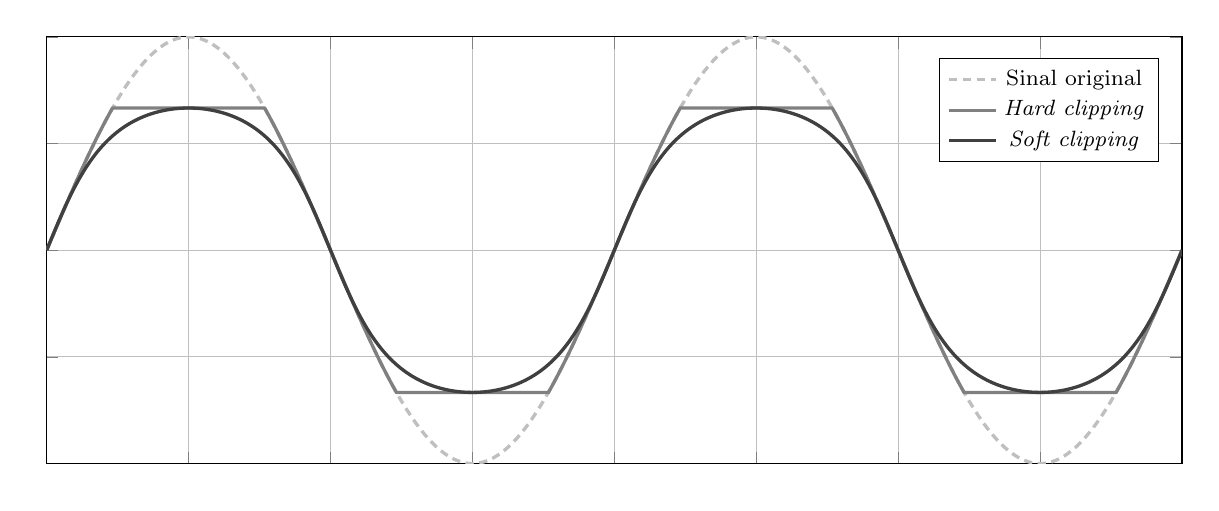
\begin{tikzpicture}[
    declare function={
        hard(\x)= (\x > 2/3) * (2/3)   +
                  and(\x <= 2/3, \x >= -2/3) * (\x) +
                  (\x < -2/3) * (-2/3);
        }
    ]

    \begin{axis}[
        ymin=-1, ymax=1, ytick={-1,-0.5,0,0.5,1},
        xmin=0, xmax=4, xtick={0,0.5,1,1.5,2,2.5,3,3.5,4},
        grid=major,
        samples=1001,
        width=16cm,
        height=7cm,
        domain=0:4,
        yticklabel=\empty,
        xticklabel=\empty,
        legend style={font=\footnotesize, at={(0.98,0.95)}, anchor=north east}
    ]
        \addplot[very thick, lightgray, densely dashed] {sin(deg(pi*x))};
        \addlegendentry{Sinal original}
        \addplot[very thick, gray] {hard(sin(deg(pi*x)))};
        \addlegendentry{\textit{Hard clipping}}
        \addplot[very thick, darkgray] {2/3 * rad(atan(tan(deg(1)) * sin(deg(pi*x))))};
        \addlegendentry{\textit{Soft clipping}}
    \end{axis}
\end{tikzpicture}